{\begin{abstract}
本章では,例題を用いたPolylibの使用法について説明します.
\end{abstract}
%

\graphicspath{{./fig_tutorial/}}

%
\section{サンプルモデルによるチュートリアル}
Polylibの利用方法を説明するために,以下のサンプルモデルを考えます.

各物体形状にはそれぞれ名前が付いており,時間発展計算の時刻ステップに応じて物体形状が移動する
物体についてはその移動計算式が分かっているものとします.

\begin{figure}[H]
 \centering
 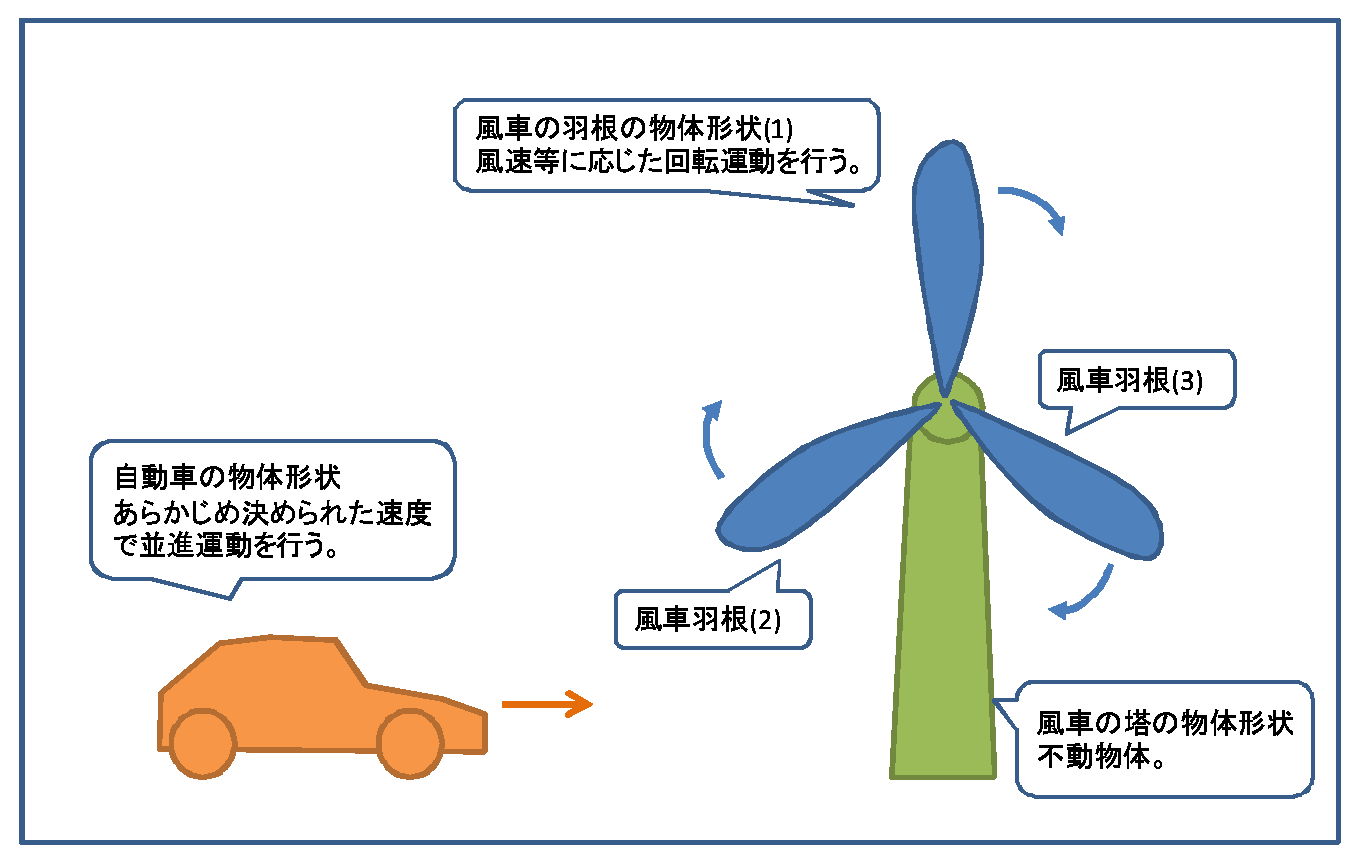
\includegraphics[scale=0.5]{clip007.eps}\\
 \caption{サンプルモデル}
\end{figure}


%
\subsection{物体形状のグルーピング}

Polylibでは物体形状ごとに,PolylgonGroupクラスインスタンスとして管理します.

PolylgonGroupクラスは,PolylgonGroupクラス同士による階層構造が表現可能です.

ライブラリユーザは,複数のPolygonGroupインスタンスを纏めて,概念的なグループを
表現することができます.

サンプルモデルについて,以下のようなグループ階層構造を定義することとします.

\begin{figure}[H]
 \centering
 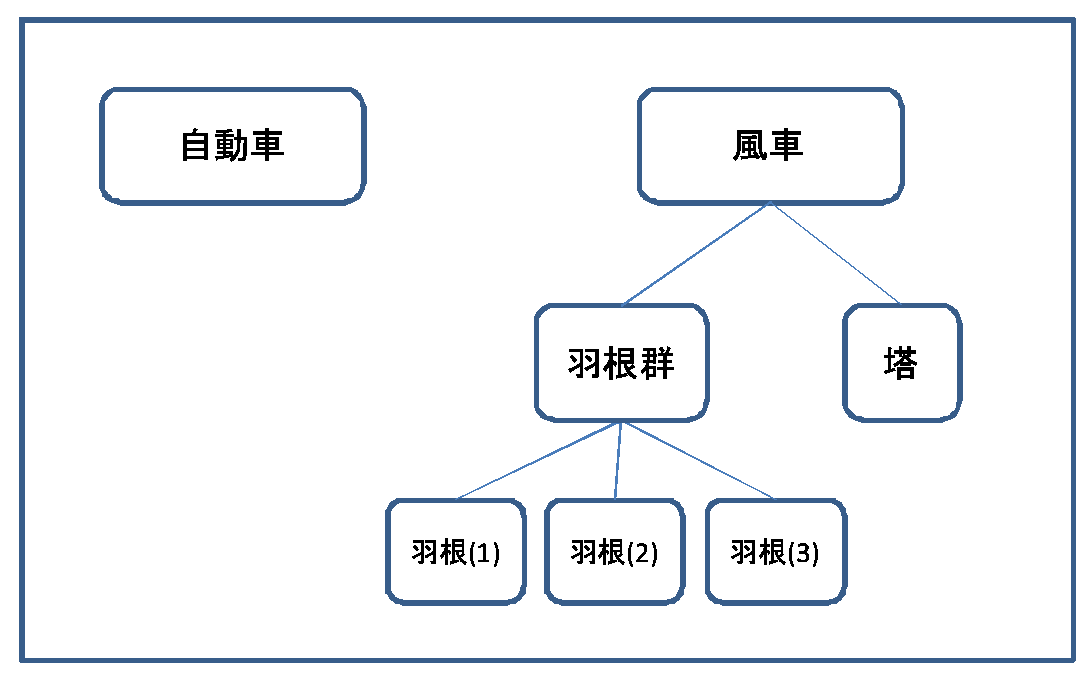
\includegraphics[scale=0.5]{clip008.eps}\\
 \caption{サンプルモデルのグループ階層構造}
\end{figure}

概念的なグループは,PolygonGroupクラスで表現することができます.特有の属性値を持
つグループや,物体形状が移動するようなグループは,PolygonGroupを派生させたユーザ
定義クラスで表現します.

サンプルモデルの風車の塔のような不動物体については,特に追加の属性などがなければ,
PolygonGroupクラスで表現します.

上記のグループ階層構造図をPolygonGroupクラスとユーザ定義の派生クラスを割り当てたも
のを下図に示します.(グループ名称もascii文字表現としました)

\begin{figure}[H]
 \centering
 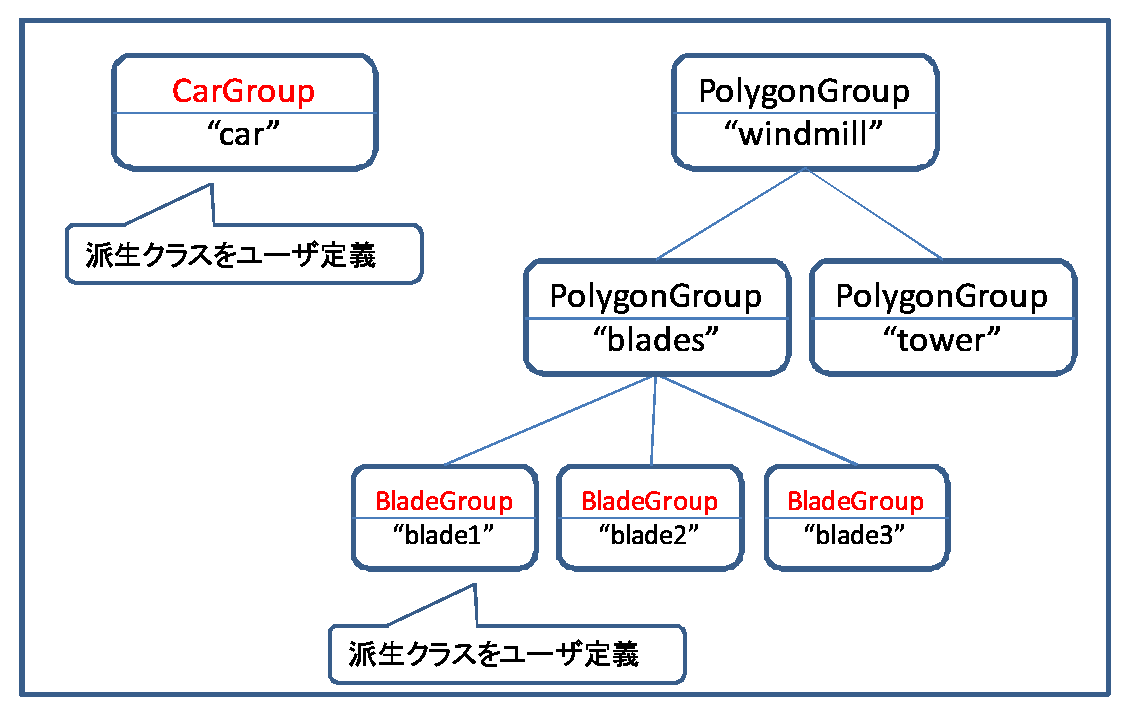
\includegraphics[scale=0.5]{clip009.eps}\\
 \caption{グループ階層構造図}
\end{figure}

%
\subsection{PolygonGroup派生クラスの定義}

ライブラリユーザは,PolygonGroupクラスを派生させた継承クラスを定義することができ
ます.

派生させることの意義は以下2点です.

\begin{itemize}
 \item 当該のポリゴングループに任意の属性値,メソッドを定義したいとき
 \item 当該のポリゴングループの座標移動計算式を定義したいとき
\end{itemize}

サンプルモデルでは,"car"が並行移動,"blade1","blade2","blade3"がそれぞれ回転移動
しますので,継承クラスを定義します.

\begin{figure}[H]
 \centering
 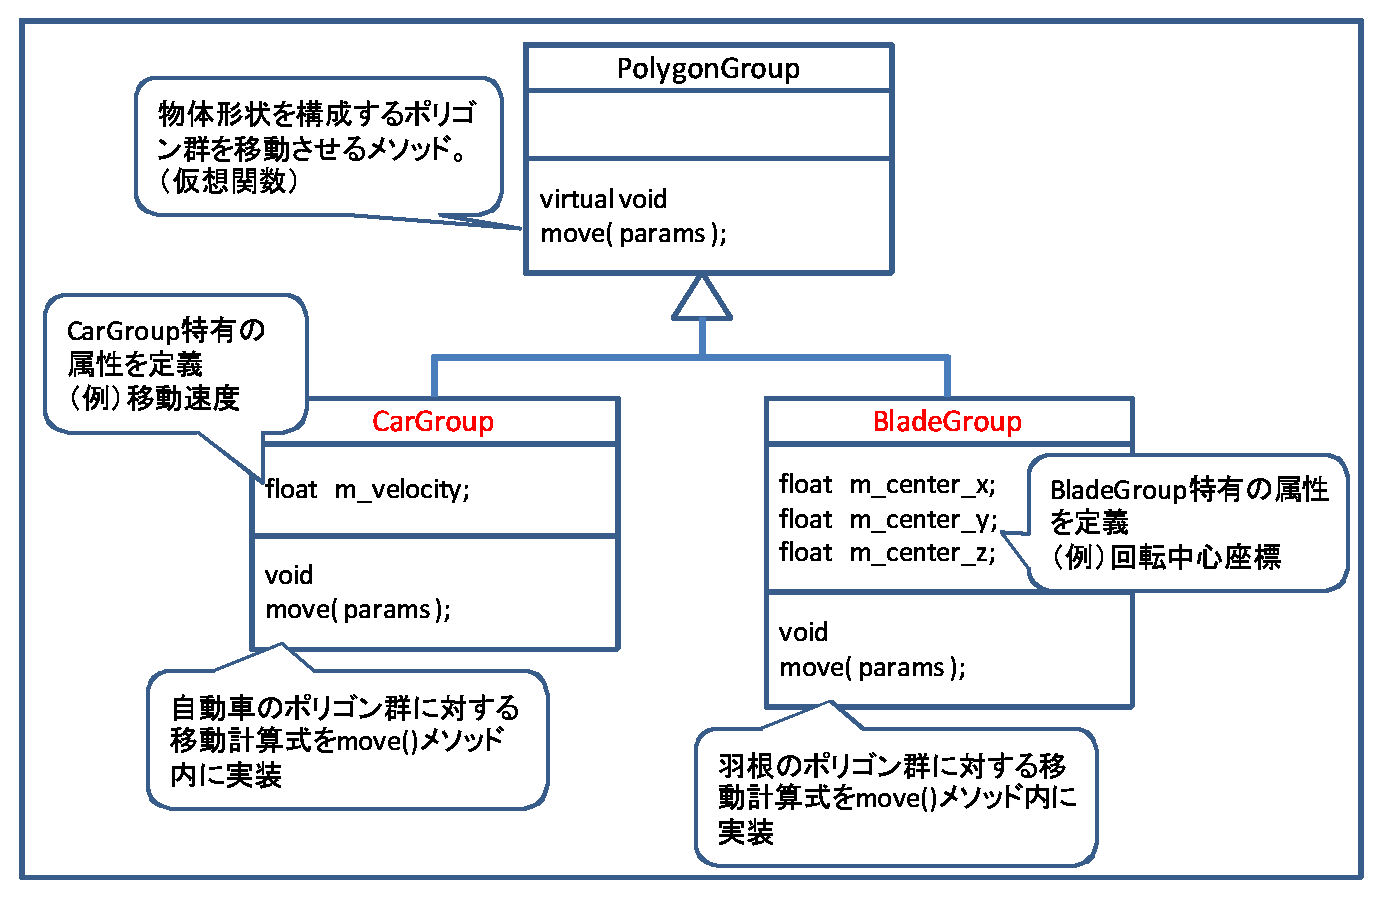
\includegraphics[width=13cm]{clip010.eps}\\
 \caption{PolygonGroupと派生クラス}
\end{figure}

派生クラスで追加した属性値は,整数,実数,文字列のいずれかであれば,グループ階層構
造構築メソッドPolygonGroup::build\_group\_tree()をオーバライドすることで,初期化ファイル
から値を取得することが可能です.CarGroupの追加属性float m\_velocityの値を取得する
CarGroup::build\_group\_tree()は以下のようになります.

\begin{program}
POLYLIB_STAT CarGroup::build_group_tree(
	Polylib			*polylib,
	PolygonGroup		*parent,
	const PolylibCfgElem	*elem
) {
	const PolylibCfgParam *att;

	// CarGroupクラスで追加定義した変数m_velocityに値を設定
	att = elem->first_param("velocity");
	if (att == NULL) {
		// エラー処理
		PL_ERROSH << "CarGroup::build_group_tree:[ERROR] velocity not found." 
			 << endl;
		return PLSTAT_CONFIG_ERROR;
	}
	m_velocity = att->get_real_data();

	// 基底クラスの属性値読み込み
	POLYLIB_STAT stat = PolygonGroup::build_group_tree(polylib, parent, elem);
	return stat;
}
\end{program}

また,追加属性をデータセーブ時にPolylib初期化ファイルに書き込むために,
PolygonGroup::mk\_param\_tag()メソッドをオーバーライドする必要があります.CarGroupの追加
属性float m\_velocityの値をPolylib初期化ファイルに保存するCarGroup:: mk\_param\_tag()は以下
のようになります.

\begin{program}
POLYLIB_STAT CarGroup::mk_param_tag(
	xmlNodePtr	elem,
	string		now,
	string		format,
	string		rank_no
){  
	POLYLIB_STAT	stat;

	// class_nameタグ作成
	stat = PolylibConfig::mk_param_tag(elem,
			PolygonGroup::ATT_NAME_CLASS, get_class_name().c_str());
	if (stat != PLSTAT_OK)	return PLSTAT_NG;

	// velocityタグ作成
	stat = PolylibConfig::mk_param_tag(elem, "velocity", m_velocity);
	if (stat != PLSTAT_OK)	return PLSTAT_NG;

	// 基底クラスが管理するタグ作成
	stat = PolygonGroup::mk_basic_tag(elem, now, format, rank_no);
	if (stat != PLSTAT_OK)	return PLSTAT_NG;

	return PLSTAT_OK;
}
\end{program}

ポリゴン群の座標移動計算式は,PolygonGroup::move()メソッドをオーバーライドして実装します.
たとえば並行移動を行うCarGroup::move()メソッドは以下のようになるでしょう.
\pagebreak
\begin{program}
POLYLIB_STAT
CarGroup::move(PolylibMoveParams&   params)
{
    // 引数チェック
    if (params.m_current_step == params.m_next_step)  return PLSTAT_OK;
    if (params.m_current_step > params.m_next_step)   return PLSTAT_NG;
    if (params.m_delta_t <= 0.0)                       return PLSTAT_NG;

    // 移動量
    // X軸方向に1stepあたりparams.m_delta_t × m_velocity だけ移動するものとする.
    float move_pos = (params.m_next_step - params.m_current_step) * 
                                         this->m_velocity * params.m_delta_t;

    // 三角形リストを取得
    std::vector<PrivateTriangle*>* tria_list = m_polygons->get_tri_list();
    std::vector<PrivateTriangle*>::iterator it;

    // 三角形リスト内の全ての三角形について頂点座標を更新
    for (it=tria_list->begin(); it!=tria_list->end(); it++) {
        PrivateTriangle *tria = (*it);
        Vec3f             *last_vtx = tria->get_vertex();
        Vec3f              moved_vtx[3];

        // X座標(t[0])のみ更新
        moved_vtx[0].t[0] = last_vtx[0].t[0] + move_pos;
        moved_vtx[1].t[0] = last_vtx[1].t[0] + move_pos;
        moved_vtx[2].t[0] = last_vtx[2].t[0] + move_pos;
        moved_vtx[0].t[1] = last_vtx[0].t[1];
        moved_vtx[1].t[1] = last_vtx[1].t[1];
        moved_vtx[2].t[1] = last_vtx[2].t[1];
        moved_vtx[0].t[2] = last_vtx[0].t[2];
        moved_vtx[1].t[2] = last_vtx[1].t[2];
        moved_vtx[2].t[2] = last_vtx[2].t[2];

        // 移動後の頂点座標を設定.法線ベクトルも再計算
        tria->set_vertexes( moved_vtx, true, false );
    }

    // 頂点座標が移動したことにより,KD木の再構築が必要.
    // 要再構築フラグを立てる.
    m_need_rebuild = true;

    return PLSTAT_OK;
}
\end{program}

実装したmove()メソッドで実際に三角形ポリゴン頂点座標が移動した場合,move()メソッド
内で,PolygonGroup::m\_need\_rebuildフラグをtrueにセットしなければならないことに注意
してください.このフラグをtureにしないとKD木の再構築が行われないため,
Polylib::search\_polygons()メソッドが正しい検索結果を返せなくなります.

また,PolygonGroup派生クラスでは,PolygonGroup::get\_class\_name()メソッドおよび
PolygonGroup::whoami()メソッドをオーバライドして実装し,システム一意なクラス名称を
返却するようにします.これは初期化ファイルに記述するクラス名称と一致させる必要が
あります.以下にCarGroupの場合の例を示します.

\begin{program}
static std::string CarGroup::get_class_name()
{
	return "CarGroup";
}

virtual std::string CarGroup::whoami()
{
	return get_class_name();
};
\end{program}

%
\subsection{PolygonGroupFactory派生クラスの定義}

サンプルモデルでは,CarGroupとBladeGroupの2種類の派生クラスがユーザ定義されました.


Polylibフレームワーク内部でこれら派生クラスインスタンスを生成するためには,生成
方法を記述した,PolygonGroupFactory派生クラスを定義する必要があります.

ここでは,MyGroupFactoryという名前の派生クラスを定義することとします.

\begin{figure}[H]
 \centering
 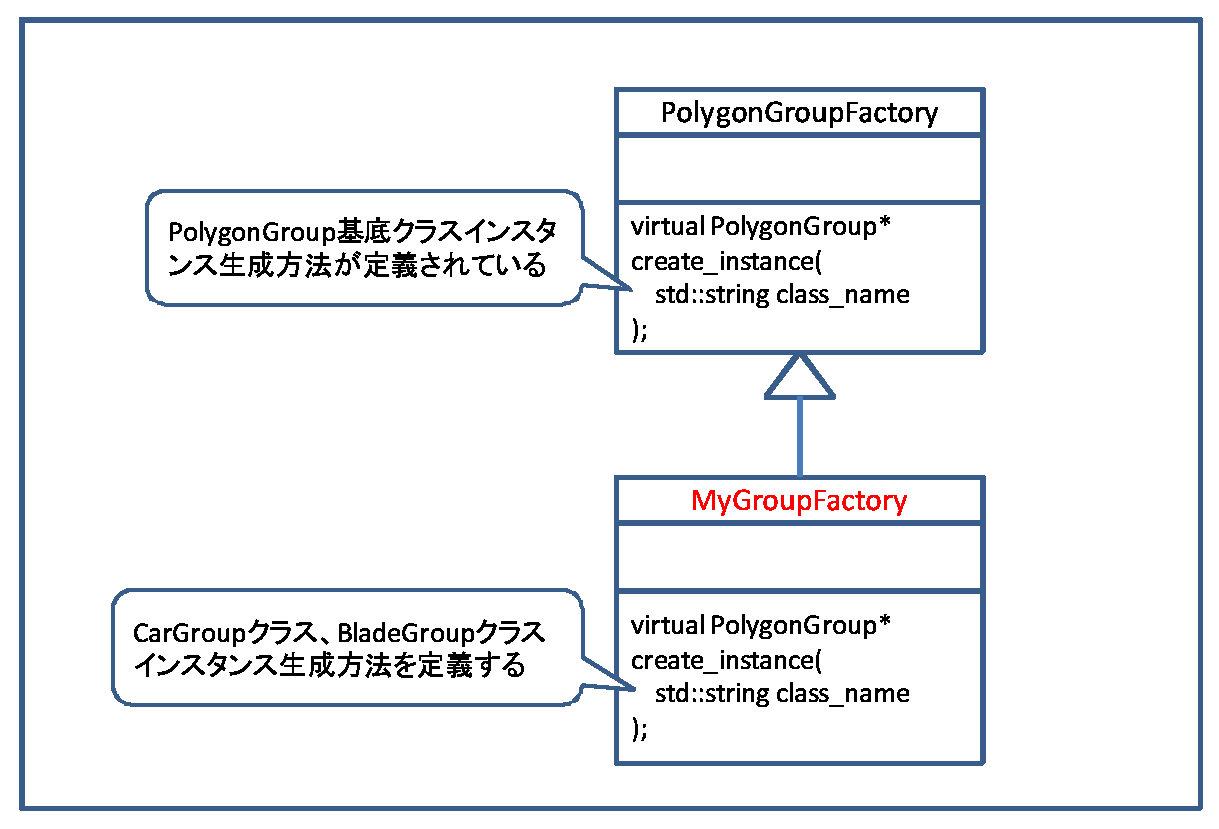
\includegraphics[width=11cm]{clip011.eps}\\
 \caption{PolygonGroupFactoryと派生クラス}
\end{figure}

Polylibには1つのPolygonGroupFactory派生クラスインスタンスしか登録できません.今回
のようにユーザ定義したPolygonGroup派生クラスが複数ある場合は,その全てのインスタンス
生成方法をMyGroupFactory::create\_instance()で実装します.以下にそのコード例を示します.

\begin{program}
PolygonGroup*
MyGroupFactory::create_instance( std::string  class_name )
{
    //---- class_nameに応じたインスタンスを生成
    // "CarGroup"の生成
    if (class_name == CarGroup::get_class_name()) {
         return new CarGroup();
    }
    // "BladeGroup"の生成
    if (class_name == BladeGroup::get_class_name()) {
         return new BladeGroup();
    }
    else {
         // 基底クラスのcreate_instanceに移譲
         return PolygonGroupFactory::create_instance(class_name);
    }
}
\end{program}

\pagebreak
%
\subsection{初期化ファイル}

サンプルモデルの初期化ファイルの内容を以下に示します.

\begin{program}
<?xml version="1.0"?>
<Parameter>
    <Elem name="PolygonGroup">
        <Param name="class_name" dtype="STRING" value="CarGroup"/>
        <Param name="name"       dtype="STRING" value="car"/>
        <Param name="filepath"   dtype="STRING" value="/foo/bar/car.stl"/>
        <Param name="movable"    dtype="STRING" value="true"/>
        <Param name="velocity"   dtype="REAL"   value="0.50"/>
    </Elem>
    <Elem name="PolygonGroup">
        <Param name="class_name" dtype="STRING" value="PolygonGroup"/>
        <Param name="name"       dtype="STRING" value="windomill"/>
        <Elem name="PolygonGroup">
            <Param name="class_name" dtype="STRING" value="PolygonGroup"/>
            <Param name="name"       dtype="STRING" value="blades"/>
            <Elem name="PolygonGroup">
                <Param name="class_name" dtype="STRING" value="BladeGroup"/>
                <Param name="name"       dtype="STRING" value="blade1"/>
                <Param name="filepath"   dtype="STRING" value="./blade1.stl"/>
                <Param name="movable"    dtype="STRING" value="true"/>
                <Param name="center_x"   dtype="REAL"   value="0.0"/>
                <Param name="center_y"   dtype="REAL"   value="123.45"/>
                <Param name="center_x"   dtype="REAL"   value="345.67"/>
            </Elem>
            <Elem name="PolygonGroup">
                <Param name="class_name" dtype="STRING" value="BladeGroup"/>
                <Param name="name"       dtype="STRING" value="blade2"/>
                <Param name="filepath"   dtype="STRING" value="./blade2.stl"/>
                <Param name="movable"    dtype="STRING" value="true"/>
                <Param name="center_x"   dtype="REAL"   value="0.0"/>
                <Param name="center_y"   dtype="REAL"   value="123.45"/>
                <Param name="center_x"   dtype="REAL"   value="345.67"/>
            </Elem>
            <Elem name="PolygonGroup">
                <Param name="class_name" dtype="STRING" value="BladeGroup"/>
                <Param name="name"       dtype="STRING" value="blade3"/>
                <Param name="filepath"   dtype="STRING" value="./blade3.stl"/>
                <Param name="movable"    dtype="STRING" value="true"/>
                <Param name="center_x"   dtype="REAL"   value="0.0"/>
                <Param name="center_y"   dtype="REAL"   value="123.45"/>
                <Param name="center_x"   dtype="REAL"   value="345.67"/>
            </Elem>
        </Elem>
        <Elem name="PolygonGroup">
            <Param name="class_name" dtype="STRING" value="PolygonGroup"/>
            <Param name="name"       dtype="STRING" value="tower"/>
            <Param name="filepath"   dtype="STRING" value="./tower.stl"/>
        </Elem>
    </Elem>
</Parameter>
\end{program}

\pagebreak

%
\subsection{メインプログラム}

以上のサンプルモデルを前提としたMPIPolylibを利用するメインプログラム例を以下に示します.

\begin{program}
#include <stdio>
#include "mpi.h"
#include "MPIPolylib.h"
#include "CarGroup.h"
#include "BladeGroup.h"
#include "MyGroupFactory.h"

using namespace std;
using namespace PolylibNS;

// 領域分割情報構造体定義
struct MyParallelInfo {
    float          bpos[3];  // 基準座標
    unsigned int bbsize[3];  // 計算領域ボクセル数
    unsigned int gcsize[3];  // ガイドセル領域ボクセル数
    float            dx[3];  // ボクセルサイズ
};

// 4並列を前提とした領域分割データ
static MyParallelInfo myParaInfos[4] = {
    {{-1100, -1800, -1800}, {18, 18, 18}, {1, 1, 1}, {100, 100, 100} },
    {{-1100,     0, -1800}, {18, 18, 18}, {1, 1, 1}, {100, 100, 100} },
    {{-1100, -1800,     0}, {18, 18, 18}, {1, 1, 1}, {100, 100, 100} },
    {{-1100,     0,     0}, {18, 18, 18}, {1, 1, 1}, {100, 100, 100} }
};

int main( int argc, char** argv )
{
    int             rank;
    unsigned int  step;
    POLYLIB_STAT  stat;
    PolylibMoveParams params;

    // MPI初期化
    MPI_Init( &argc, &argv );
    MPI_Comm_rank( MPI_COMM_WORLD, &rank );

    cout << "Starting program on rank:" << rank << endl;

    //---- MPIPolylibの初期化処理 -----
    // MPIPolylibインスタンス取得
    MPIPolylib *p_polylib = MPIPolylib::get_instance();

    // ユーザ定義ファクトリークラスを登録
    p_polylib->set_factory( new MyGroupFactory() );

    // 自PEの並列実行関連初期化情報の設定
    stat = p_polylib->init_parallel_info( MPI_COMM_WORLD,
                                    myParaInfos[rank].bpos,
                                    myParaInfos[rank].bbsize,
                                    myParaInfos[rank].gcsize,
                                    myParaInfos[rank].dx
                                );
    if( stat != PLSTAT_OK ) return -1;

    // データロード
    stat = p_polylib->load_rank0( "./polylib_config.xml" );
    if( stat != PLSTAT_OK ) return -1;

    // 時間発展計算ループ(100ステップ実行)
    for( step=0; i<100; step++ ){

        // 現在ステップでの計算実行…
        {
            // 必要なポリゴン情報を検索して取得
            vector<Triangle*>* trias =
                 p_polylib->search_polygons(/*検索条件を設定*/);

            // 検索結果ベクタの後始末
            delete trias;
        }

        // 次計算ステップへ進むためにポリゴン情報を更新
        // moveパラメタセットを設定
        PolylibMoveparams params;
        parmas.m_current_step = step;
        params.m_next_step     = step+1;
        params.m_delta_t       = 1.0;

        // move実行
        stat = p_polylib->move(params);
        if( stat != PLSTAT_OK ) return -1;

        // migrate実行
        stat = p_polylib->migrate();
        if( stat != PLSTAT_OK ) return -1;
    }

    // 各ランク毎にデータセーブ.STLはアスキー形式で出力.
    string fname;
    stat = p_polylib->save_parallel( &fname, "", "stl_a" );
    if( stat != PLSTAT_OK ) return -1;
    cout << "saved filename:" << fname << endl;

    // MPI終了処理
    MPI_Finalize();
    return 0;
}
\end{program}